% (c) 2012 Claudio Carboncini - claudio.carboncini@gmail.com
% (c) 2012 Dimitrios Vrettos - d.vrettos@gmail.com
\chapter{Espressioni letterali e valori numerici}
\section{Lettere}
\subsection{Lettere per esprimere formule}
\begin{exrig}
 \begin{esempio}
 In tutte le villette a schiera di recente costruzione del nuovo quartiere Stella, vi è un
terreno rettangolare di larghezza~$12\unit{m}$ e lunghezza~$25\unit{m}$. Quanto misura la superficie del terreno?
\begin{center}
 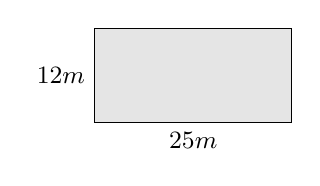
\begin{tikzpicture}[x=5mm, y=5mm,font=\small]
\definecolor{area}{gray}{0.9}
\draw [fill=area] (0,0) rectangle (5,2.4); 

\node[below] at (2.5,0) {$25\unit{m}$};
\node [left] at (0,1.2) {$12\unit{m}$};

\end{tikzpicture}
\end{center}

Il prodotto delle dimensioni rappresenta la misura richiesta:~$S=(25\cdot 12)\unit{m}^{2}=300\unit{m}^2$.
 \end{esempio}
\end{exrig}

Il semplice problema che abbiamo risolto è relativo ad un caso particolare; quel terreno con
quelle dimensioni. Ma se le dimensioni fossero diverse?

La procedura per determinare la misura della superficie ovviamente è sempre la stessa e la possiamo esprimere con la
formula~$A=b\cdot h$ nella quale abbiamo indicato con~$b$ la misura di una dimensione (base) e con~$h$ la misura dell'altra
dimensione (altezza), assegnate rispetto alla stessa unità di misura.

\osservazione La formula ha carattere generale e serve ogniqualvolta si chiede di determinare la superficie di un rettangolo,
note le misure delle dimensioni (base e altezza) rispetto alla stessa unità di misura.

In geometria si utilizzano tantissime formule che ci permettono di esprimere perimetro e
area delle figure piane, superficie laterale e totale e volume dei solidi. Nelle formule le lettere sostituiscono le
misure di determinate grandezze, tipiche di quella figura o di quel solido.

\ovalbox{\risolvi \ref{ese:9.1}}

\subsection{Lettere per descrivere schemi di calcolo}
\begin{exrig}
 \begin{esempio}
 L'insegnante chiede agli alunni di scrivere <<il doppio della somma di due numeri>>.

\begin{itemize*}
\item Antonella scrive:~$2\cdot (3+78)$;
\item Maria chiede <<Quali sono i numeri? Se non li conosco non posso soddisfare la richiesta>>;
\item Giulia scrive:~$2\cdot (a+b)$.
\end{itemize*}
Maria si è posta il problema ma non ha saputo generalizzare la richiesta. Antonella si è limitata ad un caso
particolare. Giulia ha espresso con una formula l'operazione richiesta dall'insegnante.
 \end{esempio}
\end{exrig}

\osservazione L'uso di lettere dell'alfabeto per indicare numeri ci permette di generalizzare uno schema di calcolo, cioè ci consente di scrivere un algoritmo.

\begin{definizione}
 Un'\emph{espressione letterale} o \emph{espressione algebrica} è uno schema di calcolo in cui compaiono numeri e lettere
legati dai simboli delle operazioni.
\end{definizione}

Per scrivere un'espressione letterale ci si deve attenere a regole precise, quelle stesse che utilizziamo per scrivere
espressioni numeriche.

Per esempio, la scrittura~``$3\cdot 4+$'' non è corretta, in quanto il simbolo~``$+$'' dell'addizione deve essere seguito da un
altro numero per completare l'operazione. Analogamente non è corretta l'espressione letterale~``$a\cdot c+$''.

Come nelle espressioni numeriche, anche nelle espressioni letterali le parentesi indicano la priorità di alcune operazioni rispetto ad altre.
La formula~$a\cdot (x+y)$ specifica ``il prodotto di un numero per la somma di altri due''. Essa è diversa da  $a\cdot x+y$
che rappresenta ``il prodotto di due numeri sommato a un terzo numero''.

\vspazio\ovalbox{\risolvii \ref{ese:9.2}, \ref{ese:9.3}}

\subsection{Lettere per esprimere proprietà}

Le proprietà delle operazioni tra numeri si esprimono con lettere per indicare che valgono per numeri
qualsiasi.
La scrittura ``$(a+b)+c=a+(b+c)$'', per esempio, esprime la proprietà associativa dell'addizione. In essa le lettere~$a$, $b$ e $c$ indicano
numeri qualsiasi. I due schemi di calcolo ci dicono che per sommare tre numeri è indifferente aggiungere alla somma
dei primi due il terzo oppure aggiungere al primo la somma degli altri due.

\vspazio\ovalbox{\risolvii \ref{ese:9.4}, \ref{ese:9.5}, \ref{ese:9.6}, \ref{ese:9.7}, \ref{ese:9.8}, \ref{ese:9.9}, \ref{ese:9.10}, \ref{ese:9.11}}

\section{Il valore numerico di un'espressione letterale}

Ogni espressione letterale rappresenta uno schema di calcolo in cui le lettere che vi compaiono sostituiscono numeri.
L'espressione letterale

\[2\cdot x^{2}+x\]

\noindent traduce una catena di istruzioni che in linguaggio naturale sono così
descritte: ``prendi un numero ($x$); fanne il quadrato ($x^2$); raddoppia quanto ottenuto ($2\cdot x^2$); aggiungi al risultato il numero preso inizialmente ($2\cdot x^{2}+x$)''.

Questa catena di istruzioni si può anche rappresentare in modo schematico
\[x\quad\rightarrow\quad x^{2}\quad\rightarrow\quad~2\cdot x^{2}\quad\rightarrow\quad~2\cdot x^{2}+x\]
e può essere usata per istruire un esecutore a ``calcolare'' l'espressione letterale
quando al posto della lettera~$x$ si sostituisce un numero.

Calcoliamo il valore dell'espressione~$2\cdot x^{2}+x$, sostituendo alla lettera $x$ il numero naturale~5.
Seguiamo la schematizzazione~$x\rightarrow x^{2}\rightarrow~2\cdot x^{2}\rightarrow~2\cdot x^{2}+x$ e otteniamo:
$5\rightarrow~25\rightarrow~50\rightarrow~55$.
Il risultato è~$55$.
Più brevemente scriviamo~$5$ nell'espressione letterale al posto di~$x$: otteniamo l'espressione numerica~$2\cdot 5^{2}+5$
il cui risultato è~$55$.

E se al posto di~$x$ sostituiamo~$-5$? Otteniamo un risultato diverso? Eseguiamo la sostituzione di $x$ con $-5$ e abbiamo: $2\cdot (-5)^{2}+(-5)=\ldots$ Lasciamo a te il calcolo finale. Ti sarai accorto che il
risultato è cambiato.

 \begin{definizione}
In un'espressione letterale le \emph{lettere} rappresentano le \emph{variabili} che assumono specifiche quantità
quando vengono sostituite da numeri.
Chiamiamo \emph{valore} di un'espressione letterale il risultato numerico che si ottiene eseguendo le operazioni indicate dallo
schema di calcolo quando alle lettere sostituiamo un determinato numero. Il valore di un'espressione letterale dipende dal \emph{valore assegnato} alle sue variabili.
\end{definizione}

D'ora in poi quando scriveremo un'espressione letterale in cui compare
l'operazione di moltiplicazione, tralasceremo il puntino fin qui usato per evidenziare l'operazione.
Così l'espressione~$5\cdot a^{2}+\dfrac{3}{8}\cdot a\cdot b-7\cdot b^{2}$ verrà scritta in modo
più compatto~$5a^{2}+\dfrac{3}{8}ab-7b^{2}$.

\begin{exrig}
 \begin{esempio}
Calcolare il valore numerico della seguente espressione:~$3a(a-b)$ per~$a=1$, $b=1$.

\emph{Svolgimento}:~$3\cdot 1\cdot (1-1)=3\cdot 1\cdot 0=0$.
\end{esempio}
 \end{exrig}

\ovalbox{\risolvii \ref{ese:9.12}, \ref{ese:9.13}, \ref{ese:9.14}, \ref{ese:9.15}, \ref{ese:9.16}, \ref{ese:9.17}, \ref{ese:9.18}, \ref{ese:9.19}, \ref{ese:9.20}, \ref{ese:9.21}, \ref{ese:9.22}}

\section{Condizione di esistenza di un'espressione letterale}
Ti proponiamo adesso alcuni casi particolari per
l'espressione~$E=\dfrac{x-y}{3x}$.

\paragraph{Caso I:} $x=1\,\wedge\, y=1\, \Rightarrow\, E=0$.
%
%\begin{center}
%\begin{tabular*}{.2\textwidth}{@{\extracolsep{\fill}}*{3}{c}}
%\toprule
%$x$ & $y$ & $E$\\
%1 & 1 & 0\\
%\bottomrule
%\end{tabular*}
%\end{center}

Il numeratore della frazione è~0, mentre il denominatore vale~3; il
calcolo finale è dunque~$\frac{0}{3}=0$.
Vi sono, secondo te, altre coppie di valori $(x;y)$ che fanno
assumere ad~$E$ quello stesso valore?

\paragraph{Caso II:} $x=0\,\wedge\, y=25\, \Rightarrow\, E=?$.
%\begin{center}
%\begin{tabular*}{.2\textwidth}{@{\extracolsep{\fill}}*{3}{c}}
%\toprule
%$x$ &$y$ &$E$\\
%0 &25 &?\\
%\bottomrule
%\end{tabular*}
%\end{center}

Invece di mettere un valore ad~$E$, abbiamo messo punto di domanda
perché in questo caso il numeratore della frazione è~$-25$ mentre
il denominatore vale~0; il calcolo finale è dunque~$-{\frac{25}{0}}$, impossibile.
Vi sono, secondo te, altre coppie di valori $(x;y)$ che rendono
impossibile il calcolo del valore per~$E$?

Non possiamo allora concludere che per ogni coppia di numeri razionali~$(x;y)$ 
l'espressione~$E$ assume un numero razionale.
Per poter calcolare il valore di~$E$ non possiamo scegliere coppie aventi~$x$ 
uguale a zero.
Scriveremo quindi come premessa alla ricerca dei valori di~$E$ la \emph{Condizione di Esistenza} ($\CE$)~$x\neq~0$.

L'esempio appena svolto ci fa capire che di fronte a
un'espressione letterale dobbiamo riflettere sullo
schema di calcolo che essa rappresenta prima di assegnare valori alle
variabili che vi compaiono.

Se l'espressione letterale presenta una divisione in cui
il divisore contiene variabili, dobbiamo stabilire la~$\CE$, 
eliminando quei valori che rendono nullo il divisore.
Per comprendere la necessità di porre le condizioni
d'esistenza ricordiamo la definizione di divisione.

Quanto fa~15 diviso~5? In forma matematica:~$15:5=3$ perché $3\cdot 5=15$. Quindi, 
generalizzando~$a:b=c$ se~$c\cdot b=a$.

Vediamo ora cosa succede quando uno dei numeri è~0:

\begin{itemize*}
 \item quanto fa~$0:5$? Devo cercare un numero che moltiplicato per~5 mi dia~0: trovo solo~0; infatti~$0\cdot 5=0$.
 \item quanto fa~$15:0$? Devo cercare un numero che moltiplicato per~0 mi dia~15:
non lo trovo; infatti nessun numero moltiplicato per~0 fa~15. Quindi,
$15:0$ è impossibile perché non esiste alcun
$x$ per il quale~$x\cdot 0=15$.
 \item quanto fa~$0:0$? Devo cercare un numero che moltiplicato per~0 mi dia~0:
non ne trovo solo uno. Infatti, qualunque numero moltiplicato per~0
fa~0. Per esempio, $0:0=33$; infatti
$33\cdot 0=0$. Ma anche~$0:0=\np{-189,6}$;
infatti~$\np{-189,6}\cdot 0=0$. E anche $0:0=0$;
infatti~$0\cdot 0=0$. 
Ancora~$0:0=10^{99}$, infatti~$10^{99}\cdot 0=0$.
Quindi~$0:0$ è indeterminato perché
non è possibile determinare un unico~$x$ tale che~$x\cdot 0=0$,
ma per qualunque valore di~$x$ si ha~$x\cdot 0=0$.
\end{itemize*}

Consideriamo l'espressione letterale~$E=\dfrac{a-b}{a+b}$ dove~$a$ e~$b$ 
rappresentano numeri razionali.
Premettiamo:

\begin{enumeratea}
 \item la descrizione a parole dello schema di calcolo:
``divisione tra la differenza di due numeri e la loro
somma'';
 \item la domanda che riguarda il denominatore: ``quand'è che la somma di
due numeri razionali dà come rislutato~0?'';
 \item la~$\CE$: ``$a$ e~$b$ non devono essere numeri opposti''.
\end{enumeratea}

Siamo ora in grado di completare la tabella:
\begin{center}
\begin{tabular*}{.8\textwidth}{l@{\extracolsep{\fill}}*{5}{c}}
\toprule
$a$ & 3 &0 & $\frac{3}{4}$ &$-{\frac{5}{8}}$ & $-{\frac{19}{2}}$ \\
$b$ & $-3$ & $-{\frac{1}{2}}$ & 0 &$\frac{5}{8}$ & $-{\frac{19}{2}}$ \\
\midrule
$E=\frac{a-b}{a+b}$ & & & & &\\
\bottomrule
\end{tabular*}
\end{center}

Dalla~$\CE$, ci accorgiamo subito che la
prima coppia e la quarta sono formate da numeri opposti, pertanto non
possiamo calcolare il valore di~$E$ ad esse relativo. L'ultima
coppia è formata da numeri uguali pertanto la loro differenza è~0, così
il numeratore si annulla e quindi il valore di~$E$ è~0. 
Per la coppia~$\left(0;-\frac{1}{2}\right)$ il valore di~$E$ è~$-1$ mentre è~1 per
la coppia~$\left(\frac{3}{4};0\right)$.
La tabella verrà quindi così completata:

\begin{center}
\begin{tabular*}{.8\textwidth}{l@{\extracolsep{\fill}}*{5}{c}}
\toprule
$a$ & 3 &0 & $\frac{3}{4}$ &$-{\frac{5}{8}}$ & $-{\frac{19}{2}}$ \\
$b$ & $-3$ & $-{\frac{1}{2}}$ & 0 &$\frac{5}{8}$ & $-{\frac{19}{2}}$ \\
\midrule
$E=\frac{a-b}{a+b}$ &impossibile & $-1$& 1& impossibile&0\\
\bottomrule
\end{tabular*}
\end{center}

Cosa succede per la coppia~$(0;0)$?

\vspazio\ovalbox{\risolvi \ref{ese:9.24}}
\newpage

 % (c) 2012 Dimitrios Vrettos - d.vrettos@gmail.com
\section{Esercizi}
\subsection{Esercizi dei singoli paragrafi}
\subsubsection*{9.1 - L'insieme dei monomi}
\begin{esercizio}
\label{ese:9.1}
Individua tra le espressioni letterali di seguito elencate, quelle che sono monomi.
\[E_{1}=35x^{2}+y^{2};\quad E_{2}=-4^{-1}ab^{4}c^{6};\quad E_{3}=\dfrac{4}{x}y^{2};\quad E_{4}=-{\frac{87}{2}}x^{2}z.\]

Per rispondere in modo corretto devo individuare quelle espressioni in
cui compare solamente la \dotfill; pertanto sono monomi \dotfill
\end{esercizio}

\begin{esercizio}
\label{ese:9.2}
Scrivi in forma normale i seguenti monomi:
\begin{multicols}{2}
 $\dfrac{4}{9}ab18c^{3}2^{-2}a^{3}b=\dfrac{\ldots }{\ldots }a^{\ldots}b^{\ldots }c^{\ldots };$

 $-x^{5}\dfrac{1}{9}y^{4}\big(-1+5\big)^{2}y^{7}=\dotfill~$
\end{multicols}
\end{esercizio}

\begin{esercizio}
\label{ese:9.3}
Nell'insieme
$M=\big\{-{\frac{34}{5}}a^{3}b\text{,~}3^{2}a^{2}b^{4}\text{,~}\frac{1}{3}ab^{3}\text{,~}a^{3}b\text{,~}-a\text{,~}7a^{2}b^{4}\text{,~}-\frac{1}{3}ab^{3}\text{,~}-89a^{3}b\big\}$,
determina i sottoinsiemi dei monomi simili e rappresentali con un diagramma di Venn.
\end{esercizio}

\subsubsection*{9.2 - Valore di un monomio}

\begin{esercizio}
\label{ese:9.4}
Calcola l'area di un triangolo che ha altezza~$h=\np{2,5}$ e base~$b=\frac{3}{4}$.
\end{esercizio}

\begin{esercizio}
 \label{ese:9.5}
 Calcola il valore dei seguenti monomi in corrispondenza dei valori indicati per ciascuna lettera.

\begin{multicols}{2}
\begin{enumeratea}
 \item $-\frac{2}{9}xz$ per $ x=\frac{1}{2} $, $z=-1$;
 \item $-\frac{8}{5}x^{2}y$ per $ x=-1 $, $y=+10$;
 \item $-\frac{1}{2}a^{2}bc^3$ per $ a=-\frac{1}{2} $, $b=\frac{3}{2},c=-1$;
 \item $\frac{7}{2}a^{3}x^{4}y^2$ per $ a=\frac{1}{2} $, $x=2$, $y=-\frac{1}{2}$;
 \item $\frac{8}{3}abc^2$ per $ a=-3 $, $b=-\frac{1}{3},c=\frac{1}{2}$.
\end{enumeratea}
\end{multicols}
\end{esercizio}


\begin{esercizio}
 \label{ese:9.6}
 Il grado complessivo di un monomio è:

\begin{enumeratea}
 \item l'esponente della prima variabile che compare nel monomio;
 \item la somma di tutti gli esponenti che compaiono sia ai fattori
numerici sia a quelli letterali;
 \item il prodotto degli esponenti delle variabili che compaiono nel monomio;
 \item la somma degli esponenti di tutte le variabili che vi compaiono.
\end{enumeratea}
\end{esercizio}


\begin{esercizio}
 \label{ese:9.7}
Due monomi sono simili se:

\begin{enumeratea}
 \item hanno lo stesso grado;
 \item hanno le stesse variabili;
 \item hanno lo stesso coefficiente;
 \item hanno le stesse variabili con rispettivamente gli stessi esponenti.
\end{enumeratea}
\end{esercizio}

\begin{esercizio}
 \label{ese:9.8}
Individua e sottolinea i monomi tra le seguenti espressioni letterali:
\[3+ab;\:-2a;\:-\frac{7}{3}ab^2;\:-(\frac{4}{3})^{3};\:a^{2}bc\cdot{\frac{-2}{a^{3}}};\:4a^{-3}b^{2}c^{5};\:-x; 8x^{4}-4x^{2};\:-y\cdot(2x^{4}+6z);\:\frac{abc^{9}}{3+7^{-2}}.\]
\end{esercizio}

\begin{esercizio}
 \label{ese:9.9}
Nel monomio~$m=-{\frac{5}{2}}a^{3}x^{2}y^{4}z^{8}$ distinguiamo: coefficiente~$=\ldots$,
parte letterale~$=\ldots$,
grado complessivo~$=\ldots$,
il grado della lettera~$x=\ldots$
\end{esercizio}

\begin{esercizio}
 \label{ese:9.10}
Motiva brevemente la verità o falsità delle seguenti proposizioni:
\TabPositions{8.5cm}
\begin{enumeratea}
 \item ``Se due monomi hanno ugual grado allora sono simili''\tab\boxV\quad\boxF\qquad perché\dotfill
 \item ``Se due monomi sono simili allora hanno lo stesso grado''\tab\boxV\quad\boxF\qquad perché\dotfill
\end{enumeratea}
\end{esercizio}

\begin{esercizio}
 \label{ese:9.11}
Quale dei diagrammi di Venn di seguito riportati rappresenta in modo corretto la seguente proposizione: <<alcune espressioni letterali non sono monomi>>.
$L$: insieme delle espressioni letterali, $M$: insieme dei monomi.
\begin{center}
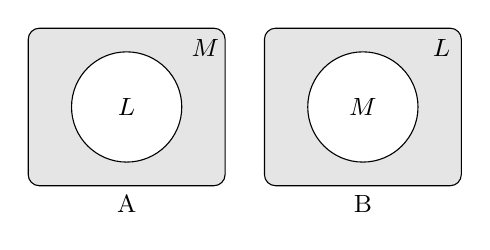
\begin{tikzpicture}[x=5mm, y=5mm,font=\small]
\definecolor{area}{gray}{0.9}
\draw [rounded corners, fill=area] (0,0) rectangle (5,4)  (4.5,3.5)node {$M$}; 
\draw[fill=white] (2.5,2) circle (1.4) node {$L$};
\node[below] at (2.5,0) {A};

\begin{scope}[xshift=30mm]
\draw [rounded corners, fill=area] (0,0) rectangle (5,4)  (4.5,3.5)node {$L$}; 
\draw[fill=white] (2.5,2) circle (1.4) node {$M$};
\node[below] at (2.5,0) {B};
\end{scope}
\end{tikzpicture}
\end{center}
\end{esercizio}

\begin{esercizio}
 \label{ese:9.12}
 Attribuisci il valore di verità alle seguenti proposizioni:
\TabPositions{11.5cm}
\begin{enumeratea}
\item Il valore del monomio~$-a$ è negativo per qualunque $a$ diverso da zero.\tab\boxV\quad\boxF
\item Il valore del monomio~$-a^{2}$ è negativo per qualunque $a$ diverso da zero.\tab\boxV\quad\boxF
\item Il monomio~$b^{6}$ è il cubo di~$b^{2}$.\tab\boxV\quad\boxF
\item L'espressione~$ab^{-1}$ è un monomio.\tab\boxV\quad\boxF
\item Il valore del monomio $ab$ è nullo per~$a = 1$ e $b =-1$.\tab\boxV\quad\boxF
\end{enumeratea}
\end{esercizio}


\subsubsection*{9.3 - Moltiplicazione di due monomi}

\begin{esercizio}
 \label{ese:9.13}
Determina il prodotto dei seguenti monomi.
\begin{multicols}{2}
\begin{enumeratea}
\spazielenx
 \item $\big(-x^{2}y^{4}\big)\cdot \bigg(-{\dfrac{8}{5}}x^{2}y\bigg)$;
 \item $\bigg(-{\dfrac{15}{28}}xy^{3}\bigg)\cdot\bigg(-\dfrac{7}{200}x^{2}y^{2}\bigg)$;
 \item $\big(a^{5}b^{5}y^{2}\big)\cdot\bigg(-\dfrac{8}{5}a^{2}y^{2}b^{3}\bigg)$;
 \item $\np{2,5}ab^{2}\cdot \bigg(-{\dfrac{1}{2}}a^{2}b\bigg)\cdot \np{1,5}a$;
 \item $\bigg(-{\dfrac{2}{9}}xz\bigg)\bigg(-{\dfrac{1}{4}}z^{3}\bigg)(27x)$;
 \item $-8\bigg(\dfrac{1}{4}x\bigg)\bigg(\dfrac{4}{5}x^{3}a^{4}\bigg)$;
 \item $5x^{3}y^{2}\cdot \bigg(-{\dfrac{1}{3}}x^{3}y^{2}\bigg)\cdot \bigg(-{\dfrac{1}{3}}\bigg)$;
 \item $6ab\cdot \bigg(-{\dfrac{1}{3}}a^{2}\bigg)\cdot {\dfrac{1}{2}ab\cdot 4a^{2}}$;
 \item $\bigg(\dfrac{7}{2}a^{3}x^{{4}}y^{2}\bigg)\cdot \bigg(-{\dfrac{8}{21}}ax^{2}y\bigg)$.
\end{enumeratea}
\end{multicols}
\end{esercizio}

\pagebreak
\begin{esercizio}
 \label{ese:9.14}
Determina il prodotto dei seguenti monomi.
\begin{multicols}{3}
\begin{enumeratea}
\spazielenx
 \item $(-2xy)\cdot (+3ax)$;
 \item $6a(-2ab)\big(-3a^{2}b^{2}\big)$;
 \item $(-1)(-ab)$;
 \item $\np{1,5}a^{2}b\cdot \bigg(-{\dfrac{2}{3}}a^{2}b\bigg)$;
 \item $-{\dfrac{7}{5}}xy^{3}\bigg(-{\dfrac{10}{3}}xy^{2}z\bigg)$;
 \item $-x\big(14x^{2}\big)$.
\end{enumeratea}
\end{multicols}
\end{esercizio}

\begin{esercizio}
 \label{ese:9.15}
Determina il prodotto delle seguenti coppie di monomi.
\begin{multicols}{3}
\begin{enumeratea}
 \item $\np{1,}\overline{{6}}xa\big(\np{1,2}xy^{2}\big)$;
 \item $\bigg(\dfrac{12}{7}m^{2}n^{3}\bigg)\bigg(-{\dfrac{7}{4}}mn\bigg)$;
 \item $\bigg(-{\dfrac{5}{4}}ax^{2}\bigg)\bigg(\dfrac{3}{10}x^{3}y\bigg)$;
 \item $12ab\bigg(-{\dfrac{1}{2}}a^{3}b^{3}\bigg)$;
 \item $\bigg(-{\dfrac{15}{8}}at^{2}\bigg)\bigg(\dfrac{6}{5}t^{3}x\bigg)$;
 \item $\bigg(\dfrac{12}{4}a^{2}n^{2}\bigg)\bigg(-{\dfrac{7}{4}}ax\bigg)$.
\end{enumeratea}
\end{multicols}
\end{esercizio}


\begin{esercizio}
 \label{ese:9.16}
Sulla base degli esercizi precedenti puoi concludere che il grado del monomio prodotto è:

\begin{enumeratea}
 \item il prodotto dei gradi dei suoi fattori;
 \item la somma dei gradi dei suoi fattori;
 \item minore del grado di ciascuno dei suoi fattori;
 \item uguale al grado dei suoi fattori.
\end{enumeratea}
\end{esercizio}

\subsubsection*{9.4 - Potenza di un monomio}
\begin{esercizio}
 \label{ese:9.17}
 Esegui le potenze indicate.
\begin{multicols}{2}
\begin{enumeratea}
\spazielenx
 \item $\bigg(-{\dfrac{3}{5}}abx^{3}y^{5}\bigg)^{3}=\dfrac{\ldots }{\ldots}a^{3}b^{3}x^{\ldots }y^{\ldots}$;
 \item $\big(-a^{4}b^{2}\big)^{7}=\ldots$;
 \item $\bigg(-3x^{3}y^{4}z\bigg)^{2}=9x^{6}y^{\ldots }z^{\ldots }$;
 \item $\bigg(\dfrac{1}{2}a^{2}bc^{5}\bigg)^{4}=\dfrac{1}{\ldots}a^{\ldots}b^{\ldots}c^{\ldots}$;
 \item $\big(a^{3}b^{2}\big)^{8}=\ldots$;
 \item $\big(-5ab^{2}c\big)^{3}=\ldots$
\end{enumeratea}
\end{multicols}
\end{esercizio}

\begin{esercizio}
 \label{ese:9.18}
 Esegui le potenze indicate.
\begin{multicols}{3}
\begin{enumeratea}
\spazielenx
 \item $\big(+2ax^{3}y^{2}\big)^{2}$;
 \item $\bigg(-{\dfrac{1}{2}}axy^{2}\bigg)^{3}$;
 \item $\bigg(\dfrac{3}{4}x^{4}y\bigg)^{3}$;
 \item $\bigg(\dfrac{2}{3}xy^{2}\bigg)^{3}$;
 \item $\bigg(-{\dfrac{1}{2}}ab\bigg)^{4}$;
 \item $\bigg(-{\dfrac{3}{2}}a^{5}\bigg)^{2}$.
\end{enumeratea}
\end{multicols}
\end{esercizio}

\begin{esercizio}
 \label{ese:9.19}
 Esegui le operazioni indicate.
\begin{multicols}{2}
\begin{enumeratea}
\spazielenx
 \item $\bigg[\big(-rs^{2}t\big)^{2}\bigg]^{3}$;
 \item $\Bigg[\bigg(-{\dfrac{1}{2}}x^{2}y^{3}\bigg)^{2}\Bigg]^{3}$;
 \item $\Bigg[\bigg(-{\dfrac{3}{2}}a^{2}b^{3}\bigg)^{2}\Bigg]^{2}$;
 \item $\big(-xy\big)^{2}\bigg(-{\dfrac{1}{2}}xy^{2}\bigg)^{3}$;
 \item $-\bigg(\dfrac{3}{2}xy^{2}\bigg)^{0}\cdot\bigg(-{\dfrac{1}{6}}xy\bigg)^{2}$;
 \item $-\bigg(-{\dfrac{1}{3}}x^{3}y^{2}\bigg)^{2}\cdot\bigg(-{\dfrac{1}{3}}\bigg)^{-3}$.
\end{enumeratea}
\end{multicols}
\end{esercizio}

\begin{esercizio}
 \label{ese:9.20}
 Esegui le operazioni indicate.
\begin{multicols}{2}
\begin{enumeratea}
\spazielenx
 \item $\bigg(\dfrac{2}{3}ab^{2}c\bigg)^{2}\cdot\big(-3ab^{3}\big)^{2}$;
 \item $\Bigg[\bigg(-{\dfrac{1}{2}}a^{2}b\bigg)^{2}\cdot{\dfrac{2}{3}a^{2}b}\Bigg]^{2}$;
 \item $\bigg(\dfrac{2}{3}x\cdot{\dfrac{1}{6}}x\cdot {\dfrac{1}{2}}x\bigg)^{2}\cdot\bigg(-{\dfrac{1}{6}}ab^{2}\bigg)^{2}$.
\end{enumeratea}
\end{multicols}
\end{esercizio}

\subsubsection*{9.5 - Divisione di due monomi}
\begin{esercizio}
 \label{ese:9.21}
Esegui le divisioni indicate e poni le~$\CE$:
\begin{multicols}{2}
\begin{enumeratea}
\spazielenx
 \item $15b^{8}:\bigg(-{\dfrac{40}{3}}b^{3}\bigg)$;
 \item $\bigg(-{\dfrac{13}{72}}x^{2}y^{5}z^{3}\bigg):\bigg(-{\dfrac{26}{27}}xyz\bigg)$;
 \item $(-a^{7}):(8a^{7})$;
 \item $\bigg(\dfrac{1}{2}a^{3}\bigg):(-4a^{5})$;
 \item $\bigg(-{\dfrac{12}{2}}a^{7}b^{5}c^{2}\bigg):(-18ab^{4}c)$;
 \item $(-34x^{5}y^{2}):(-2yz^{3})$.
\end{enumeratea}
\end{multicols}
\end{esercizio}

\begin{esercizio}
 \label{ese:9.22}
Esegui le divisioni indicate e poni le~$\CE$:
\begin{multicols}{2}
\begin{enumeratea}
 \item $21a^{3}x^{4}b^{2}:7ax^{2}b$;
 \item $a^{6}:20a^{2}$;
 \item $20ax^{4}y:2xy$;
 \item $-72a^{4}b^{2}y^{2}:(-3ab^{2})$.
\end{enumeratea}
\end{multicols}
\end{esercizio}

\begin{esercizio}
 \label{ese:9.23}
Esegui le operazioni indicate e poni le~$\CE$:
\begin{multicols}{2}
\begin{enumeratea}
 \item $48a^{5}bx:a^{2}b$;
 \item $\Bigg[-\bigg(-{\dfrac{1}{3}}x^{3}y^{2}\bigg)^{2}:\bigg(-{\dfrac{1}{3}}\bigg)\Bigg]^{2}:(x^{3}y^{2})^{2}$;
 \item $\Bigg[\dfrac{3}{5}x^{4}:\bigg(\dfrac{1}{3}x^{4}\bigg)\Bigg]\cdot\Bigg[x^{4}:\bigg(\dfrac{4}{5}x^{4}\bigg)\Bigg]$;
 \item $\bigg(\dfrac{2}{3}ab^{2}c\bigg)^{2}:(-3ab^{3})$.
\end{enumeratea}
\end{multicols}
\end{esercizio}

\subsubsection*{9.6 - Addizione di due monomi simili}
\begin{esercizio}
 \label{ese:9.24}
Determina la somma dei monomi simili~$8a^{2}b+(-{\frac{2}{3}})a^{2}b+\frac{1}{6}a^{2}b$.

La somma è un monomio \ldots\ldots\ldots agli
addendi; il suo coefficiente è dato da
$8-\frac{2}{3}+\frac{1}{6}=\ldots $, la parte letterale è~$\dotfill~$ Quindi la
somma è~$\dotfill$
\end{esercizio}

\begin{esercizio}
 \label{ese:9.25}
Determina la somma~$S=2a-3ab-a+17ab+41a$.

I monomi addendi non sono tra loro simili, modifico la scrittura
dell'operazione applicando le proprietà associativa e commutativa
in modo da affiancare i monomi simili:
\[S=2a-3ab-a+17ab+41a=(\ldots\ldots\ldots)+(\ldots\ldots\ldots)=\ldots\ldots\ldots\]
La somma ottenuta non è un \ldots\ldots\ldots\ldots\ldots
\end{esercizio}
\pagebreak
\begin{esercizio}
 \label{ese:9.26}
Esegui la somma algebrica dei seguenti monomi.
\begin{multicols}{3}
\begin{enumeratea}
 \item $6x+2x-3x$;
 \item $-3a+2a-5a$;
 \item $5a^{2}b-3a^{2}b$;
 \item $a^{2}b^{2}-3a^{2}b^{2}$;
 \item $2xy-3xy+xy$;
 \item $2y^{2}-3y^{2}+7y^{2}-4y^{2}$.
\end{enumeratea}
\end{multicols}
\end{esercizio}

\begin{esercizio}
 \label{ese:9.27}
Esegui la somma algebrica dei seguenti monomi.
\begin{multicols}{3}
\begin{enumeratea}
 \item $-2xy^{2}+xy^{2}$;
 \item $-3ax-5ax$;
 \item $5ab-2ab$;
 \item $-3xy^{2}+3xy^{2}$;
 \item $7xy^{3}-2xy^{3}$;
 \item $+2xy^{2}-4xy^{2}$.
\end{enumeratea}
\end{multicols}
\end{esercizio}

\begin{esercizio}
 \label{ese:9.28}
Esegui la somma algebrica dei seguenti monomi.
\begin{multicols}{2}
\begin{enumeratea}
 \item $\dfrac{1}{2}a^{2}-a^{2}$;
 \item $+2xy^{2}-4xy^{2}+xy^{2}$;
 \item $-5x^{2}+3x^{2}$;
 \item $\dfrac{1}{2}a+2a$;
 \item $5a^{2}b+2a^{2}b+a^{2}b-3a^{2}b-a^{2}b$;
 \item $\np{0,1}x-5x-\np{1,2}x+3x$.
\end{enumeratea}
\end{multicols}
\end{esercizio}

\begin{esercizio}
 \label{ese:9.29}
Esegui la somma algebrica dei seguenti monomi.
\begin{multicols}{2}
\begin{enumeratea}
\spazielenx
 \item $\dfrac{1}{4}a^{3}b^{2}-\dfrac{1}{2}a^{3}b^{2}$;
 \item $\dfrac{2}{3}x-\dfrac{2}{5}x-2x+\dfrac{3}{10}x$;
 \item $\dfrac{2}{5}ab-\dfrac{1}{2}ab+\dfrac{27}{2}ab-\dfrac{1}{10}ab-\dfrac{5}{2}ab$;
 \item $-\bigg(-{\dfrac{1}{2}}ax^{2}\bigg)-3ax^{2}$;
 \item $-{\dfrac{9}{2}}xy-(-xy)$;
 \item $2xy^{2}-\dfrac{3}{2}xy^{2}-xy^{2}$.
\end{enumeratea}
\end{multicols}
\end{esercizio}

\begin{esercizio}
 \label{ese:9.30}
Esegui la somma algebrica dei seguenti monomi.
\begin{multicols}{2}
\begin{enumeratea}
\spazielenx
 \item $\dfrac{1}{2}a+2a+(2a-a)-\bigg(3a-\dfrac{1}{2}a\bigg)$;
 \item $6xy^{2}+\dfrac{1}{3}xy^{2}-\dfrac{1}{4}xy^{2}-6xy^{2}$;
 \item $\dfrac{1}{2}xy^{2}+\dfrac{3}{2}xy^{2}$;
 \item $\bigg(\dfrac{2}{3}a+a\bigg)-\bigg(\dfrac{2}{3}a-a\bigg)$;
 \item $5ab-2ab+(-ab)-(+2ab)+ab$;
 \item $\np{-1,2}x^{2}+\np{0,1}x^{2}+(-5x)^{2}-(-25x)^{2}$.
\end{enumeratea}
\end{multicols}

\end{esercizio}


\begin{esercizio}
 \label{ese:9.31}
Esegui le operazioni indicate.
\begin{multicols}{2}
\begin{enumeratea}
\spazielenx
 \item $6ab-\dfrac{1}{3}a^{2}+\dfrac{1}{2}ab+4a^{2}$;
 \item $\bigg(\dfrac{1}{4}x^{2}-\dfrac{3}{4}x^{2}+x^{2}\bigg)-\bigg(-{\dfrac{1}{3}}x^{2}+\dfrac{1}{2}x^{2}\bigg)$;
 \item $-{\dfrac{4}{3}}a^{2}b^{3}-2a^{2}b^{3}+\dfrac{1}{3}a^{2}b^{3}-a^{2}b^{3}$;
 \item $\big(-xy\big)^{2}\bigg(-{\dfrac{1}{2}}xy^{2}\bigg)+\dfrac{3}{2}xy^{2}\bigg(-{\dfrac{1}{6}}xy\bigg)^{2}$.
\end{enumeratea}
\end{multicols}
\end{esercizio}

\begin{esercizio}
 \label{ese:9.32}
Esegui la somma algebrica dei seguenti monomi.

\begin{enumeratea}
\spazielenx
 \item $\dfrac{1}{2}x^{2}-2x^{2}-\bigg(-{\dfrac{1}{2}}x^{2}+\dfrac{3}{4}x^{2}-2x^{2}-\dfrac{3}{5}x^{2}\bigg)$;
 \item $5x^{3}y^{2}+\bigg(-{\dfrac{1}{3}}x^{3}y^{2}\bigg)+\bigg(-{\dfrac{1}{3}}\bigg)-\big(x^{3}y^{2}\big)+\bigg(-{\dfrac{1}{4}}x^{3}y^{2}\bigg)-\bigg(-{\dfrac{1}{3}}\bigg)$;
 \item $\bigg(2xy^{2}-\dfrac{3}{2}xy^{2}\bigg)-\big(xy^{2}+2xy^{2}-4xy^{2}\big)+\bigg(xy^{2}+\dfrac{1}{2}xy^{2}\bigg)$.
\end{enumeratea}
\end{esercizio}

\subsubsection*{9.7 - Espressioni con i monomi}
\begin{esercizio}[\Ast]
 \label{ese:9.33}
Esegui le operazioni tra monomi.

\begin{enumeratea}
 \item $\bigg(\dfrac{1}{2}a^{2}-a^{2}\bigg)\bigg(\dfrac{1}{2}a+2a\bigg)+(2a-a)\bigg(3a-\dfrac{1}{2}a\bigg)a$;
 \item $\bigg(\dfrac{2}{3}a-\dfrac{5}{2}a\bigg)a+\bigg(7a-\dfrac{1}{3}a\bigg)^{2}:2$;
 \item $\dfrac{1}{2}x^{2}\bigg(x^{2}+\dfrac{1}{2}x^{2}\bigg)-\dfrac{1}{6}x^{3}\bigg(12x-\dfrac{18}{5}x\bigg)$;
 \item $\bigg(-{\dfrac{3}{4}}x^{4}a^{2}b\bigg):\bigg(\dfrac{1}{2}x^{2}ab\bigg)+\dfrac{2}{3}x^{2}a$;
 \item $\bigg(\dfrac{1}{2}a-\dfrac{1}{4}a\bigg)^{2}:\bigg(\dfrac{3}{2}a-2a\bigg)$;
 \item $(3a-2a)(2x+2x):2a$.
\end{enumeratea}
\end{esercizio}

\begin{esercizio}[\Ast]
 \label{ese:9.34}
Esegui le operazioni tra monomi.

\begin{enumeratea}
 \item $\bigg(\dfrac{1}{4}x^{2}-\dfrac{2}{3}x^{2}+x^{2}\bigg)\bigg(-{\dfrac{1}{3}}x+\dfrac{1}{2}x\bigg)$;
 \item $\bigg(\dfrac{1}{5}x-\dfrac{5}{2}x+x\bigg)-\bigg(2x-\dfrac{8}{3}x+\dfrac{1}{4}x+x\bigg)-\dfrac{7}{60}x$;
 \item $5a+\Bigg\{-{\dfrac{3}{4}}a-\bigg[2a-\dfrac{1}{2}a+\big(3a-a\big)+\np{0,5}a\bigg]-a\Bigg\}$;
 \item $-12x^{2}\bigg(\dfrac{1}{3}x\bigg)^{2}+\bigg[\np{0,1}x^{2}\big(-5x\big)^{2}-\big(-x^{2}\big)^{2}\bigg]$;
 \item $-{\dfrac{3}{5}}x^{2}y^{2}\bigg(-{\dfrac{10}{9}}xz^{2}\bigg)(-15xy)-\np{0,}\overline{{6}}x^{4}yz\big(\np{-0,}\overline{{7}}xy^{2}z\big)$;
 \item $\dfrac{1}{2}ab^{2}c+\Bigg[\dfrac{3}{4}a^{3}b^{6}c^{3}-\bigg(-{\dfrac{1}{4}ab^{2}c}\bigg)^{3}-\bigg(-{\dfrac{1}{2}ab^{2}}\bigg)^{2}\bigg(-{\dfrac{1}{16}ab^{2}c^{3}}\bigg)\Bigg]:%
 \bigg(-{\dfrac{5}{4}a^{2}b^{4}c^{2}}\bigg)$.
\end{enumeratea}
\end{esercizio}

\begin{esercizio}[\Ast]
 \label{ese:9.35}
Esegui le operazioni tra monomi.

\begin{enumeratea}
 \item $\bigg(2xy^{2}-\dfrac{3}{2}xy^{2}\bigg)-\big(xy^{2}+2xy^{2}-4xy^{2}\big)+\bigg(xy^{2}+\dfrac{1}{2}xy^{2}\bigg)$;
 \item $\dfrac{1}{4}x^{4}y^{2}-\bigg[\dfrac{3}{2}x^{5}y^{4}:\bigg(\dfrac{1}{2}xy\bigg)^{2}-3x^{3}y^{2}\bigg]%
 \bigg(-{\dfrac{1}{3}}x\bigg)+\bigg(-{\dfrac{1}{2}}x^{2}y\bigg)^{2}$;
 \item $a^{2}-\Bigg\{a-\bigg[2\bigg(\dfrac{a}{2}-\dfrac{a}{3}\bigg)\bigg]\Bigg\}^{2}+%
 \bigg(\dfrac{2}{3}a+a\bigg)\bigg(\dfrac{2}{3}a-a\bigg)$;
 \item $\bigg[\bigg(-{\dfrac{1}{2}}a^{2}b\bigg)^{2}\cdot\bigg(-{\dfrac{2}{3}}b^{2}\bigg)^{2}-%
 \bigg(+{\dfrac{1}{3}}b^{3}a^{2}\bigg)^{2}\bigg]:\bigg(\dfrac{2}{3}a-\dfrac{1}{6}a+\dfrac{1}{2}a\bigg)+\bigg(-{\dfrac{1}{6}}ab^{2}\bigg)^2%
 \bigg(-{\dfrac{2}{5}}ab^2\bigg)$;
 \item \begin{multline*}
 \Bigg[\bigg(2x+\dfrac{7}{4}x\bigg)^{2}:\bigg(\dfrac{1}{3}x+x+\dfrac{3}{4}x\bigg)\Bigg]^{2}%
:\bigg(18x-\dfrac{9}{2}x+\dfrac{27}{2}x\bigg)+\\
 +\bigg[\bigg(-{\dfrac{2}{3}}abx\bigg)^{2}-\bigg(\dfrac{1}{3}abx\bigg)^{2}\bigg]:(a^{2}b^{2}x)-x;
 \end{multline*}
 \item \begin{multline*}
 \bigg(\dfrac{1}{4}xy^{2}\bigg)\bigg(-{\dfrac{16}{5}}x^{2}y\bigg)-8x^{2}y^{2}\bigg(-2xy\bigg)%
 -\dfrac{2}{5}x\bigg(-{\dfrac{5}{3}}x^{2}\bigg)\bigg(+3y^{3}\bigg)+\\
 +\bigg(\dfrac{12}{7}xy^{2}\bigg)\bigg(-{\dfrac{7}{4}}x^{2}y\bigg)+\dfrac{9}{5}x^{3}y^{3}.
 \end{multline*}
\end{enumeratea}
\end{esercizio}


\begin{esercizio}[\Ast]
 \label{ese:9.36}
Esegui le operazioni tra monomi.

\begin{enumeratea}
 \item $\dfrac{2}{3}a^{2}b-\bigg[3a-\dfrac{1}{3}a^{2}b-\bigg(\dfrac{2}{5}a+\dfrac{1}{2}a-3a\bigg)+\bigg(\dfrac{2}{5}a^{2}b+\dfrac{1}{2}a^{2}b-2a^{2}b\bigg)\bigg]%
 -\dfrac{1}{10}a^{2}b+\dfrac{51}{10}a$;
 \item $\bigg(\dfrac{1}{3}x+\dfrac{1}{2}x-2x\bigg)\bigg(-{\dfrac{1}{2}x^{2}}\bigg)+\bigg(\dfrac{3}{4}x^{2}-2x^{2}\bigg)\bigg(-{\dfrac{3}{5}x}\bigg)%
 -\dfrac{4}{3}\bigg(x^{3}+\dfrac{1}{2}x^{3}\bigg)$;
 \item \begin{multline*}
 \Bigg[\dfrac{3}{5}ab^{2}+\dfrac{1}{2}b-ab^{2}\cdot\bigg(-{\dfrac{3}{10}}+\dfrac{4}{5}-\dfrac{1}{2}\bigg)-2b+\dfrac{3}{2}b+\dfrac{1}{15}ab^{2}\Bigg]^{2}:\\%
:\bigg[\bigg(b+\dfrac{3}{2}b\bigg)^{2}-\dfrac{5}{10}b^{2}+\dfrac{1}{2}b^{2}\bigg]\cdot\bigg(-{\dfrac{5}{2}ab}\bigg)^{2};
 \end{multline*}
 \item $\bigg[\bigg(\dfrac{3}{2}xy\bigg)^{2}\cdot(\dfrac{4}{15}y\bigg)^{2}-\bigg(\dfrac{3}{2}xy^{2}\bigg)^{2}\cdot\bigg(\dfrac{2}{3}\bigg)^{3}%
 +\dfrac{8}{75}x^{2}y^{4}\bigg]:\bigg(\dfrac{10}{3}x^{2}y\bigg)$;
 \item $\bigg(\dfrac{1}{2}x+2x\bigg)\bigg(\dfrac{1}{2}x-2x\bigg)\bigg(\dfrac{1}{4}x^{2}-4x^{2}\bigg)-\dfrac{1}{4}x\bigg(\dfrac{27}{4}x^{3}-\dfrac{61}{3}x^{3}\bigg)%
 -16(x^{4}+x^{4})-\dfrac{1}{12}x^{2}\cdot x^{2}+\dfrac{1}{8}x^{4}$.
\end{enumeratea}
\end{esercizio}


\begin{esercizio}
 \label{ese:9.37}
Assegnati i monomi:
$m_{{1}}=\dfrac{3}{8}a^{2}b^{2}$, $m_{2}=-{\dfrac{8}{3}}ab^{3}$, $m_{3}=-3a$, $m_{{4}}=-{\dfrac{1}{2}}b$ e~$m_{{5}}=2b^{3}$.
Calcola il risultato delle seguenti operazioni, ponendo le opportune~$\CE$:
\begin{multicols}{3}
\begin{enumeratea}
 \item $m_{{1}}\cdot m_{2}\cdot (m_{{4}})^{2}$;
 \item $-m_{2}\cdot m_{{1}}\cdot (m_{3})^{2}\cdot m_{{5}}$;
 \item $(m_{3}\cdot m_{{4}})^{2}-m_{{1}}$;
 \item $m3\cdot m_{{5}}-m_{2}$;
 \item $m_{2}:m_{3}+m_{{5}}$;
 \item $m_{{1}}:m_{2}$.
\end{enumeratea}
\end{multicols}
\end{esercizio}


\begin{esercizio}
 \label{ese:9.38}
Quando sottraiamo due monomi opposti otteniamo:
\begin{enumeratea}
\item il doppio del primo termine;
\item il doppio del secondo termine;
\item il monomio nullo;
\item 0.
\end{enumeratea}
\end{esercizio}

\begin{esercizio}
 \label{ese:9.39}
Quando dividiamo due monomi opposti otteniamo:
\begin{center}
\boxA\quad~$-1$
\quad\boxB\quad~0
\quad\boxC\quad~1
\quad\boxD\quad il quadrato del primo monomio
\end{center}
\end{esercizio}

\begin{esercizio}
 \label{ese:9.40}
Attribuisci il valore di verità alle seguenti proposizioni:
\TabPositions{11cm}
\begin{enumeratea}
 \item la somma di due monomi opposti è il monomio nullo \tab\boxV\quad\boxF
 \item il quoziente di due monomi simili è il quoziente dei loro coefficienti \tab\boxV\quad\boxF
 \item la somma di due monomi è un monomio \tab\boxV\quad\boxF
 \item il prodotto di due monomi è un monomio \tab\boxV\quad\boxF
 \item l'opposto di un monomio ha sempre il coefficiente negativo \tab\boxV\quad\boxF
\end{enumeratea}
\end{esercizio}

\begin{esercizio}[\Ast]
 \label{ese:9.41}
Un quadrato è formato da~9~quadrati più piccoli, tutti di lato $ 2x $. Determina perimetro e area del quadrato.
\end{esercizio}

\begin{esercizio}[\Ast]
 \label{ese:9.42}
Di un triangolo equilatero di lato $ a $ si raddoppiano due lati e si dimezza il terzo lato, si ottiene un triangolo \ldots\ldots\ldots Qual è la differenza tra i perimetri dei due triangoli?
\end{esercizio}

\subsubsection*{9.8 - Massimo Comune Divisore e minimo comune multiplo tra monomi}

\begin{esercizio}
 \label{ese:9.43}
Vero o falso?

\TabPositions{9cm}
\begin{enumeratea}
\item $12a^{3}b^{2}c$ è un multiplo di~$abc$ \tab\boxV\quad\boxF
\item $2xy$ è un divisore di~$x^{2}$ \tab\boxV\quad\boxF
\item $2a$ \ è divisore di~$4ab$ \tab\boxV\quad\boxF
\item $-5b^{2}$ è divisore di~$15ab$ \tab\boxV\quad\boxF
\item $8ab$ è multiplo di~$a^{2}b^{2}$ \tab\boxV\quad\boxF
\item $12a^{5}b^{4}$ è multiplo di~$60a^{5}b^{7}$ \tab\boxV\quad\boxF
\item $5$ è divisore di~$15a$ \tab\boxV\quad\boxF
\end{enumeratea}
\end{esercizio}

\begin{esercizio}
 \label{ese:9.44}
Vero o falso?

\TabPositions{10cm}
\begin{enumeratea}
\item il~$\mcm$ fra monomi è divisibile per tutti i monomi dati \tab\boxV\quad\boxF
\item il~$\mcd$ fra monomi è multiplo di almeno un monomio dato \tab\boxV\quad\boxF
\item il~$\mcm$ è il prodotto dei monomi tra di loro \tab\boxV\quad\boxF
\end{enumeratea}
\end{esercizio}

\begin{esercizio}[\Ast]
 \label{ese:9.45}
Calcola il~$\mcm$ e il~$\mcd$ dei seguenti gruppi di monomi.

\begin{enumeratea}
 \item $14x^{3}y^{2}$, $xy$ e~$4x^{3}y^{4}$;
 \item $xyz^{5}$e~$x^{3}y^{2}z^{2}$;
 \item $4ab^{2}$, $a^{3}b^{2}$ e~$5ab^{5}$.
\end{enumeratea}
\end{esercizio}

\begin{esercizio}
 \label{ese:9.46}
Calcola il~$\mcm$ e il~$\mcd$ dei seguenti gruppi di monomi.

\begin{enumeratea}
 \item $2a^{2}bc^{3}$, $ab^{4}c^{2}$ e~$24a^{3}bc$;
 \item $6a^{2}x$, $2ax^{3}$ e~$4x^{2}c^{3}$;
 \item $30ab^{2}c^{4}$, $5a^{2}c^{3}$ e~$12abc$.
\end{enumeratea}
\end{esercizio}

\begin{esercizio}
 \label{ese:9.47}
Calcola il~$\mcm$ e il~$\mcd$ dei seguenti gruppi di monomi.

\begin{enumeratea}
 \item $x^{2}y^{4}z^{2}$, $xz^{3}$ e~$24y^{2}z$;
 \item $4a^{2}y$, $y^{3}c$ e~$15ac^{5}$;
 \item $13xyc^{2}$, $x^{2}y^{3}c^{2}$ e~$6c^{4}$.
\end{enumeratea}
\end{esercizio}

\begin{esercizio}[\Ast]
 \label{ese:9.48}
Calcola il~$\mcm$ e il~$\mcd$ dei seguenti gruppi di monomi.

\begin{enumeratea}
 \item $a^{n}b^{m}z^{2m+1}$, $a^{3n}b^{m+3}$ e~$a^{4n}b^{m+4}$;
 \item $-2xy^{3}z$, $-6x^{3}yz$ e~$8x^{3}z$;
 \item $\frac{1}{4}ab^{2}c$, $-3a^{2}b^{2}c$ e~$-{\frac{1}{2}}ab^{2}c^{2}$;
 \item $\frac{2}{3}x^{2}y^{2}$, $\frac{1}{6}xy^{2}$ e~$\frac{2}{5}xyz^{2}$.
\end{enumeratea}
\end{esercizio}

\begin{esercizio}
 \label{ese:9.49}
Dati i monomi~$3xy^{2}$ e~$xz^{3}$

\begin{enumeratea}
\item calcola il loro~$\mcd$;
\item calcola il loro~$\mcm$;
\item verifica che il loro prodotto è uguale al prodotto tra il loro~$\mcm$ e il loro~$\mcd$;
\item verifica che il loro~$\mcd$ è uguale al quoziente tra il loro prodotto e il loro~$\mcm$.
\end{enumeratea}
\end{esercizio}

\subsection{Risposte}

\paragraph{9.33.} d)~$-\frac{5}{6}ax^{2}$.
\paragraph{9.34.} a)~$\frac{7}{72}x^{3}$,\quad b)~$-2x$, \quad c)~$-\frac{3}{4}a$, \quad d)~$\frac{1}{6}x^{4}$, \quad f)~$-\frac{1}{8}ab^{2}c$.
\paragraph{9.35.} a)~$3xy^{2}$,\quad b)~$\frac{3}{2}x^{4}y^{2}$, \quad c)~0, \quad d)~$-\frac{1}{90}a^{3}b^{6}$, \quad e)~$\frac{49}{48}x$, \quad f)~$16x^{3}y^{3}$.
\paragraph{9.36.} a)~$2a^{2}b$,\quad b)~$-\frac{2}{3}x^{3}$, \quad c)~$\frac{4}{9}a^{4}b^{4}$, \quad d)~$-\frac{3}{25}y^{3}$.
\paragraph{9.41.} $24x$;\:$36x^2$.
\paragraph{9.42.} $\frac{3}{2}a$.
\paragraph{9.45.} a)~$28x^{3}y^{4};\:xy$,\quad b)~$x^{3}y^{2}z^{5};\:xyz^{2}$, \quad c)~$20a^{3}b^{5};\:ab^{2}$.
\paragraph{9.48.} a)~$a^{4n}b^{m+4}z^{2m+1};\:a^{n}b^{m}$,\quad b)~$24x^{3}y^{3}z;\:2xz$,\quad c)~$a^{2}b^{2}c^{2};\:ab^{2}c$,\quad d)~$x^{2}y^{2}z^{2};\:xy$.


\cleardoublepage
